\documentclass[english,a4paper,11pt,oneside,onecolumn]{book}

\usepackage{pst-all}
 \usepackage{pgfplotstable}
 
 \usepackage{url}
 \usepackage{braket}
 \usepackage{tikz}
\usepackage{mathtools}
\usetikzlibrary{arrows.meta}
\usepackage[utf8]{inputenc}

\setlength{\topmargin}{-1cm}
\setlength{\headsep}{.5cm}
%\setlength{\footskip}{1.0cm}
\setlength{\textheight}{24.7cm}
\setlength{\textwidth}{17cm}
\setlength{\evensidemargin}{-.5cm}
\setlength{\oddsidemargin}{-.5cm}

\usepackage{lastpage}



\usepackage{babel}
\usepackage{slantsc}
\usepackage{array}

\usepackage{listings}
\usepackage{minitoc}
\usepackage{float}
\usepackage{fancybox}
\usepackage{amsmath}
\newcommand{\EE}{\mathrm{I\!E\!}}
\newcommand{\bmat}[1]{\mbox{\boldmath $ #1 $}}
\usepackage{fancyheadings}
\usepackage{fancyhdr}

\usepackage{shadethm}


\usepackage{ifpdf}
\usepackage{amsthm}

\usepackage{lastpage}

%% for inserting programming code
\usepackage{minted}

%%%%%%%%%%%%%%%

\fancypagestyle{plain}{}

\pagestyle{fancy}
\lhead{\copyright Jayprakash Asolkar}
\rhead{Page \thepage /\pageref{LastPage}}
%\chead{\thepage}
\chead{\today}
\lfoot{School of Computer Science \& Statistics}
\rfoot{Trinity College Dublin, Ireland}
\cfoot{}
%%%%%%%%%%%%%%%

                

\ifpdf                                                                                           
 \pdfcompresslevel=9

\usepackage{color}


\newcommand{\red}[1]{{\color{red} #1}}
\newcommand{\solution}[1]{{\color{red} #1}}

 \usepackage[pdftex]{hyperref}                  
  \hypersetup{backref,bookmarks=true,pdfpagemode=Fullscreen,linkcolor=black,colorlinks=true,urlcolor=blue}

\pdfinfo{
/Title ()
/Author ()
/Date (2016)
/Subject ()
/Keywords ()
	}
 \usepackage{graphicx}
\graphicspath{{}}
\DeclareGraphicsExtensions{.jpg,.tif,.pdf,.mps,.png}
\else                                                                                            
  \usepackage{graphicx}           
\graphicspath{{}}
\DeclareGraphicsExtensions{.eps}                                                               
\fi                        

\renewcommand{\baselinestretch}{1.5}

\usepackage{fourier}

%\usepackage[scaled]{uarial} # not available anymore
\usepackage{tgheros}
\renewcommand*\familydefault{\sfdefault} 
\usepackage[T1]{fontenc}






%%%%%%%%%%%%%%%%%%%%%%%%%%%%%%%%%%%%%%%%

\begin{document}
\renewcommand{\footrulewidth}{1pt}







\begin{titlepage}
	\centering
	

\includegraphics[width=.8\linewidth]{trinity-common-use.jpg}\par\vspace{2cm}
% * <dahyotr@tcd.ie> 2018-02-02T15:45:10.514Z:
%
% ^.
	\vspace{2cm}
	{\huge\bfseries Quantum Machine Learning Data Classification\par}
	\vspace{1cm}
	{\scshape \par}
	\vspace{2cm}
	{\Large by Jayprakash Asolkar \par}
	{\Large Supervisor: Prof. Rozenn Dahyot \par}
 \vspace{1cm}
{\scshape 
A Dissertation submitted to the University of Dublin,\\
in partial fulfilment of the requirements for the degree of\\
Master of Science in Computer Science (Intelligent Systems),\\
School of Computer Science \& Statistics\\ 
Trinity College Dublin, Ireland\\
}
\end{titlepage}

\clearpage

%%%%%%%%%%%%%%%%%%%%%%%%%%%%%%%%%%%%%%%%%%%%%%%%%%%%%%%%%%%%
\chapter*{Declaration}

I declare that this thesis has not been submitted as an exercise for a degree at this or
any other university and it is entirely my own work.

\vspace{0.5cm}

\noindent I agree to deposit this thesis in the University$\textquotesingle$s open access institutional repository or
allow the library to do so on my behalf, subject to Irish Copyright Legislation and
Trinity College Library conditions of use and acknowledgement.


\vspace{3cm}
\begin{flushright}

\begin{tabular}{l}
% signature\\
\hline
Jayprakash Asolkar\\
\end{tabular}

\vspace{0.5cm}

\today
\end{flushright}



%%%%%%%%%%%%%%%%%%%%%%%%%%%%%%%%%%%%%%%%%%%%%%%%%%%%%%%%%%%%
\chapter*{Forewords}

This is an example  of a possible  template designed for TCD students for writing a report in \LaTeX written by  Prof R. Dahyot\footnote{\url{https://www.scss.tcd.ie/Rozenn.Dahyot/}}. 

\chapter*{Acknowledgments}

To be completed.

\chapter*{Abstract}
To be completed.

\tableofcontents

\listoffigures

\listoftables


%%%%%%%%%%%%%%%%%%%%%%%%%%%%%%%%%%%%%%%%%%%%%%%%%%%%%%%%%%%%
%

\chapter{Introduction} 

To be completed.




%%%%%%%%%
\chapter{Background Research}
\label{sec:soa}

The development of Quantum Mechanics over the last century has paved the way for the new paradigm of computation. Paul Benioff with his research on Quantum Information and Quantum mechanical model of Turing Machines pioneered the field of Quantum Computing. Quantum computation is based on the postulates of quantum mechanics which define the way quantum systems behave. In the last couple of decades, many theoretical quantum algorithms have been developed which suggest a possible superiority of quantum computers over their classical counterparts. This section discusses, in brief, the basics of quantum computing required to build more complex algorithms which can help to solve some of the challenging problems faced by classical computers. Furthermore, it gives an overview of state of the art applications of quantum computing across various domains.

\section{Quantum Bit}
\label{sec:qubit}

\noindent The most basic unit of computation for classical computers is a bit (binary digit) which is used to store and process information. Quantum computers make use of a similar unit of information called Quantum Bit or Qubit. Unlike the classical bit which can represent either a zero state or one state at any given time, a qubit can simultaneously be in a superposition state of both $\ket{0}$ and $\ket{1}$ state. More precisely, the state of a single qubit is a unit vector in a 2-dimensional complex vector space called Hilbert Space. The special states $\ket{0}$ and $\ket{1}$, of the qubit vector are called the orthonormal basis of the Hilbert space. Any arbitrary state $\ket{$\psi$}$ of the qubit can be defined as a linear combination of the basis vectors.
\begin{equation}\label{eq:1}
    \ket{\psi} = \alpha\ket{0} + \beta\ket{1} \hspace{25}where\hspace{10} \braket{\psi|\psi} = |\psi|^2 = 1
\end{equation}

\noindent In the equation \ref{eq:1}, \(\alpha\) and \(\beta\) are complex numbers and \(|\alpha|^2\), \(|\beta|^2\) are the probabilities of measuring the qubit in $\ket{0}$ or $\ket{1}$ basis states respectively. The matrix representation of the arbitrary qubit state $\ket{$\psi$}$ and basis states $\ket{0}$, $\ket{1}$ is given by equation \ref{eq:2}. On an ideal quantum computer, measurement of a qubit in $\ket{0}$ basis state yields the binary digit 0, hundred percent of the times. Similarly there is 100\% probability of a qubit in $\ket{1}$ state resulting in the measurement of binary digit 1. 
\begin{equation}\label{eq:2}
\ket{\psi} = 
\begin{bmatrix}
\alpha\\
\beta
\end{bmatrix}\hspace{25}
\ket{0} = 
\begin{bmatrix}
1\\
0
\end{bmatrix}\hspace{25}
\ket{1} = 
\begin{bmatrix}
0\\
1
\end{bmatrix}
\end{equation}
The pure state of a qubit can also be thought as a point residing on the surface of the Bloch Sphere. Figure \ref{fig:bloch1} shows the Bloch sphere representation of the qubit state vector.

\begin{figure}[H]
\centering
 \begin{tikzpicture}[line cap=round, line join=round, >=Triangle]
  \clip(-2.19,-2.49) rectangle (2.66,2.58);
  \draw [shift={(0,0)}, lightgray, fill, fill opacity=0.1] (0,0) -- (56.7:0.4) arc (56.7:90.:0.4) -- cycle;
  \draw [shift={(0,0)}, lightgray, fill, fill opacity=0.1] (0,0) -- (-135.7:0.4) arc (-135.7:-33.2:0.4) -- cycle;
  \draw(0,0) circle (2cm);
  \draw [rotate around={0.:(0.,0.)},dash pattern=on 3pt off 3pt] (0,0) ellipse (2cm and 0.9cm);
  \draw (0,0)-- (0.70,1.07);
  \draw [->] (0,0) -- (0,2);
  \draw [->] (0,0) -- (-0.81,-0.79);
  \draw [->] (0,0) -- (2,0);
  \draw [dotted] (0.7,1)-- (0.7,-0.46);
  \draw [dotted] (0,0)-- (0.7,-0.46);
  \draw (-0.08,-0.3) node[anchor=north west] {$\varphi$};
  \draw (0.01,0.9) node[anchor=north west] {$\theta$};
  \draw (-1.01,-0.72) node[anchor=north west] {$\mathbf {\hat{x}}$};
  \draw (2.07,0.3) node[anchor=north west] {$\mathbf {\hat{y}}$};
  \draw (-0.5,2.6) node[anchor=north west] {$\mathbf {\hat{z}=|0\rangle}$};
  \draw (-0.4,-2) node[anchor=north west] {$-\mathbf {\hat{z}=|1\rangle}$};
  \draw (0.4,1.65) node[anchor=north west] {$|\psi\rangle$};
  \scriptsize
  \draw [fill] (0,0) circle (1.5pt);
  \draw [fill] (0.7,1.1) circle (0.5pt);
 \end{tikzpicture}
\caption{Bloch Sphere} \label{fig:bloch1}
\end{figure}

\noindent North and south poles of the sphere represent $\ket{0}$, $\ket{1}$ states respectively. As shown in equation \ref{eq:3}, by ignoring the global phase, angles \(\theta\) and \(\varphi\) can be used to define any arbitrary state of a qubit. 

\begin{equation}\label{eq:3}
    \ket{\psi} = cos\hspace{2}\dfrac{\theta}{2}\hspace{2}\ket{0} + e^i^\varphi \hspace{2}sin\hspace{2}\dfrac{\theta}{2}\hspace{2}\ket{1}
\end{equation}

\noindent Real quantum computers make use of atoms, trapped ions, electrons, photons to realize quantum bits. Physically $\ket{0}$ and $\ket{1}$ states may correspond to polarization of a photon or the alignment of nuclear spins.

\section{Multiple Qubits and Entanglement}
\label{sec:multiQubit}
A single qubit alone is not sufficient to perform quantum computation. The power of quantum computers lies in the use of registers of qubits and their co-related states. Using n qubits in superposition state of $\ket{0}$ and $\ket{1}$, for eg. \(\dfrac{\ket{0} + \ket{1}}{\sqrt{2}}\), we can represent \(2^n\) states simultaneously in a multi-qubit system. However, it should be noted that measurement of the state of a qubit collapses the state to one of the basis states and destroys the quantum information. Hence, at any given time, only a single state can be retrieved through measurement of a quantum system. This remains a challenge in developing efficient quantum algorithms.

\noindent A multiple qubit system with n qubits has \(2^n\) computational basis states. These basis states of a multi-qubit system can be obtained by using tensor product of the basis states of individual qubits (For eg. $\ket{00}$ = $\ket{0}$\otimes$\ket{0}$). Equation \ref{eq:4} represents an arbitrary state $\ket{\psi}$ in 2-qubit system. 

\begin{equation}\label{eq:4}
    \ket{\psi} = \alpha\ket{00} + \beta\ket{01} + \gamma\ket{10} + \delta\ket{11} \hspace{15} where \hspace{10} |\alpha|^2 + |\beta|^2 + |\gamma|^2 + |\delta|^2 = 1
\end{equation}

\noindent An important feature of multi-qubit quantum system is the ability to prepare entangled states of two or more qubits. The states of 2 entangled qubits affect each other even if the qubits are separated by a long distance. The entangled state \(\dfrac{\ket{00} + \ket{11}}{\sqrt{2}}\) is called the Bell state or EPR pair and is the basic ingredient of multiple quantum algorithms. The terminology entanglement of two qubits specifies that the measurement of the state of only a single qubit among the EPR pair is sufficient to predict the outcome of measurement of the second qubit with absolute certainty.

\section{Quantum Gates}
\label{sec:qGates}
For any meaningful computation, the ability to manipulate states of the qubits is essential. Various quantum gates are the means to linearly transform the state vector of a single qubit or register of multiple qubits. Quantum computers make use of lasers, magnetic fields or other technologies to physically alter the qubit state.

\noindent Similar to classical logic gates namely AND, OR, XOR etc., quantum computers make use of quantum gates which linearly change the qubit state vector. The Pauli-X gate is similar to classical NOT gate and acts on a single qubit to change the state from \(\ket{0}\) to \(\ket{1}\) and vice versa. The Pauli-X gate is represented in matrix format as shown in equation \ref{eq:5}.
\begin{equation}\label{eq:5}
X = 
\begin{bmatrix}
0 & 1\\
1 & 0
\end{bmatrix}
\end{equation}

\noindent The quantum Pauli-X gate acts linearly on the arbitrary state $\ket{\psi}$ to swap the measurement probabilities of \(\ket{0}\) and \(\ket{1}\) vectors. The equation \ref{eq:6} shows the application of the Pauli-X gate as the inner product of the gate with the state vector.
\begin{equation}\label{eq:6}
X\ket{\psi} = \alpha X \ket{0} + \beta X \ket{1} = 
\alpha
\begin{bmatrix}
0 & 1\\
1 & 0
\end{bmatrix}
\begin{bmatrix}
1\\
0
\end{bmatrix} + 
\beta
\begin{bmatrix}
0 & 1\\
1 & 0
\end{bmatrix}
\begin{bmatrix}
0\\
1
\end{bmatrix} = 
\alpha
\begin{bmatrix}
0\\
1
\end{bmatrix} + 
\beta
\begin{bmatrix}
1\\
0
\end{bmatrix} =
\alpha\ket{1} + \beta\ket{0}
\end{equation}

\noindent The Pauli-Y and Pauli-Z gates are other two gates in the Pauli set and both of these act on a single qubit. Another important single qubit gate is the Hadamard gate. The Hadamard gate creates an equal superposition of both the computational basis states. Matrix representation of Pauli-Y, Pauli-Z and Hadamard gates is given by equation \ref{eq:7}. 

\begin{equation}\label{eq:7}
Y = 
\begin{bmatrix}
0 & -i\\
i & 0
\end{bmatrix}
\hspace{25}
Z = 
\begin{bmatrix}
1 & 0\\
0 & -1
\end{bmatrix}
\hspace{25}
H = \dfrac{1}{\sqrt{2}}
\begin{bmatrix}
1 & 1\\
1 & -1
\end{bmatrix}
\end{equation}

\noindent Quantum computation also makes use of gates acting on states of multiple qubits. A 4x4 CNOT gate acts on a register of 2 qubits. One of the qubits acts as the control qubit whereas another qubit in the set is called the target qubit. Based on the state of control qubit, the CNOT gate acts on the target qubit to flip its state. If the control qubit is in the state \(\ket{0}\) then the CNOT gate does nothing to the target qubit and its state remains unchanged, whereas if the control qubit is in the state \(\ket{1}\), the CNOT gate acts as a X gate on the target qubit. The dimensions of the matrix of a multi-qubit gate acting on n qubits is \(2^n\)x\(2^n\).

\begin{equation}\label{eq:8}
U_C_N_O_T = 
\begin{bmatrix}
1 & 0 & 0 & 0\\
0 & 1 & 0 & 0\\
0 & 0 & 0 & 1\\
0 & 0 & 1 & 0
\end{bmatrix}
\end{equation}

\noindent All quantum gates are unitary matrices i.e. the hermitian conjugate or adjoint of the gate matrix is also the inverse of the matrix. A hermitian conjugate is obtained by flipping the given matrix over its diagonal and changing the sign of the imaginary parts of the complex numbers. This constraint on the quantum gates makes them reversible. Hence, information about the input to the quantum gate never gets lost unlike the classical logic gates. Equation \ref{eq:9} is true for every quantum gate U and depicts that applying any gate twice on input qubit states restores the original quantum state. Also, unitary matrices maintain the normalization condition of the qubit state given by \(|\alpha|^2\) + \(|\beta|^2\) = 1.

\begin{equation}\label{eq:9}
UU^\dagger = I \hspace{25} where \hspace{5}U^\dagger = Adjoint(U)
\end{equation}

\noindent As shown in equations \ref{eq:10} and \ref{eq:11}, the reversibility of quantum gates can be verified for any of the gates discussed so far. 
\begin{equation}\label{eq:10}
HH = 
\dfrac{1}{\sqrt{2}}
\begin{bmatrix}
1 & 1\\
1 & -1
\end{bmatrix}
\hspace{10}
\dfrac{1}{\sqrt{2}}
\begin{bmatrix}
1 & 1\\
1 & -1
\end{bmatrix}
=
\begin{bmatrix}
1 & 0\\
0 & 1
\end{bmatrix}
=I
\end{equation}
\begin{equation}\label{eq:11}
HH\ket{\psi} = I \ket{\psi} = \ket{\psi}
\end{equation}

\noindent Effect of any arbitrary quantum gate on the state of a qubit can be thought of as a rotation of the state vector around different axes in the Bloch sphere. Additionally, any arbitrary transformation of the qubit state can be achieved by using combination of few basic gates.

\section{Quantum Circuits}
\label{sec:qCirc}
Quantum algorithms are depicted using the circuit model of computation. A quantum circuit comprises of register of qubits, quantum gates and measurements in classical bits. Logically, the simplest possible quantum circuit is a quantum wire which retains the state of a qubit over a period of time or a communication channel. However, this is the most difficult quantum circuit to implement physically, as the state of a qubit gets easily affected by its environment, corrupting the quantum information. 

\begin{figure}[H]
    \centering
    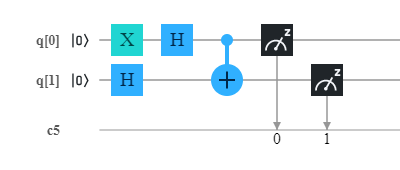
\includegraphics[scale=0.7]{quantumCircuitExample.png}
    \caption{An example of quantum circuit visualized using IBMQ circuit composer}
    \label{fig:qCircEx}
\end{figure}

\noindent Figure \ref{fig:qCircEx} shows the composition of a quantum circuit. Two qubits \(q_0\) and \(q_1\) of the quantum register are prepared in the \(\ket{0}\) basis state. The qubit \(q_0\) is passed through the quantum wire across the X and Hadamard gates, whereas the qubit \(q_1\) is passed through the quantum wire across the Hadamard gate. The 2-qubit CNOT gate uses \(q_0\) as the control qubit and works on the target qubit \(q_1\). Finally both the qubits are measured on the classical channel c5. After the measurement, the state of each of the qubits collapses to the computational basis state. More complex circuits can be built in similar way to realize various quantum algorithms which can utilize quantum properties such as superposition and entanglement.

\section{Quantum Computing - Hype and Promises}
\label{sec:qHype}
The Deutsch-Jozsa algorithm was one of the first algorithms which showed that the quantum computers can be used to achieve exponential speedups using quantum parallelism over the best known classical algorithms. Shor's prime factoring algorithm was a catalyst for the growing interest in quantum computing and quantum cryptography. It makes use of the efficiency of quantum fourier transform to find prime factors of given number N in polynomial time. No known classical algorithm exists that can acheive the same task polynomially even on best super computers. Grover's search algorithm provides quadratic speed improvement for searching a database with unsorted entries.\\

\noindent Currently available quantum computers are still in early stages of development and thus restrict the practical verification of many theoretical algorithms which claim quantum supremacy. Furthermore, these machines are prone to errors due to environmental interference and decoherence, which is an active area of research in the field of quantum computation. However, steady growth of number of qubits and power of quantum computers, cloud access to physical systems and arrival of various software development kits for programmers all around the world to develop and test new algorithms, are some of the encouraging factors for research in this area.\\

\noindent The no-cloning theorem of quantum bits states that quantum information stored in one qubit can not be copied to another qubit without altering the state of the original qubit. This phenomenon has implications in the field of quantum cryptography and future of data security. Quantum chemistry is a major field of research as quantum computers can simulate quantum systems efficiently. Classical computers require exponentially increasing resources for simulation of such quantum information. Multiple companies have recognized the vast potential of quantum computers and are investing heavily in the field. Quantum machine learning, image processing, data analysis are few more fields that are gaining interest from scholars all around the globe.

\section{Quantum Machine Learning}
\label{sec:qml}


\section{Quantum Data Classification}
\label{sec:qmlDataClass}

%%%%%%%%
\chapter{Work to date}
\label{sec:wtd}


%%%
\chapter{Future work}
\label{sec:fw}


%%%%%%%%%%%%%%%%%%%%%%%%%%%%%%%%%%%%
\addcontentsline{toc}{chapter}{Bibliography}
\nocite{}
\bibliographystyle{plain}
\bibliography{ReferenceList}

\appendix
\chapter{my appendix}



\end{document}
